% Options for packages loaded elsewhere
\PassOptionsToPackage{unicode}{hyperref}
\PassOptionsToPackage{hyphens}{url}
%
\documentclass[
]{article}
\usepackage{amsmath,amssymb}
\usepackage{iftex}
\ifPDFTeX
  \usepackage[T1]{fontenc}
  \usepackage[utf8]{inputenc}
  \usepackage{textcomp} % provide euro and other symbols
\else % if luatex or xetex
  \usepackage{unicode-math} % this also loads fontspec
  \defaultfontfeatures{Scale=MatchLowercase}
  \defaultfontfeatures[\rmfamily]{Ligatures=TeX,Scale=1}
\fi
\usepackage{lmodern}
\ifPDFTeX\else
  % xetex/luatex font selection
\fi
% Use upquote if available, for straight quotes in verbatim environments
\IfFileExists{upquote.sty}{\usepackage{upquote}}{}
\IfFileExists{microtype.sty}{% use microtype if available
  \usepackage[]{microtype}
  \UseMicrotypeSet[protrusion]{basicmath} % disable protrusion for tt fonts
}{}
\makeatletter
\@ifundefined{KOMAClassName}{% if non-KOMA class
  \IfFileExists{parskip.sty}{%
    \usepackage{parskip}
  }{% else
    \setlength{\parindent}{0pt}
    \setlength{\parskip}{6pt plus 2pt minus 1pt}}
}{% if KOMA class
  \KOMAoptions{parskip=half}}
\makeatother
\usepackage{xcolor}
\usepackage[margin=1in]{geometry}
\usepackage{color}
\usepackage{fancyvrb}
\newcommand{\VerbBar}{|}
\newcommand{\VERB}{\Verb[commandchars=\\\{\}]}
\DefineVerbatimEnvironment{Highlighting}{Verbatim}{commandchars=\\\{\}}
% Add ',fontsize=\small' for more characters per line
\usepackage{framed}
\definecolor{shadecolor}{RGB}{248,248,248}
\newenvironment{Shaded}{\begin{snugshade}}{\end{snugshade}}
\newcommand{\AlertTok}[1]{\textcolor[rgb]{0.94,0.16,0.16}{#1}}
\newcommand{\AnnotationTok}[1]{\textcolor[rgb]{0.56,0.35,0.01}{\textbf{\textit{#1}}}}
\newcommand{\AttributeTok}[1]{\textcolor[rgb]{0.13,0.29,0.53}{#1}}
\newcommand{\BaseNTok}[1]{\textcolor[rgb]{0.00,0.00,0.81}{#1}}
\newcommand{\BuiltInTok}[1]{#1}
\newcommand{\CharTok}[1]{\textcolor[rgb]{0.31,0.60,0.02}{#1}}
\newcommand{\CommentTok}[1]{\textcolor[rgb]{0.56,0.35,0.01}{\textit{#1}}}
\newcommand{\CommentVarTok}[1]{\textcolor[rgb]{0.56,0.35,0.01}{\textbf{\textit{#1}}}}
\newcommand{\ConstantTok}[1]{\textcolor[rgb]{0.56,0.35,0.01}{#1}}
\newcommand{\ControlFlowTok}[1]{\textcolor[rgb]{0.13,0.29,0.53}{\textbf{#1}}}
\newcommand{\DataTypeTok}[1]{\textcolor[rgb]{0.13,0.29,0.53}{#1}}
\newcommand{\DecValTok}[1]{\textcolor[rgb]{0.00,0.00,0.81}{#1}}
\newcommand{\DocumentationTok}[1]{\textcolor[rgb]{0.56,0.35,0.01}{\textbf{\textit{#1}}}}
\newcommand{\ErrorTok}[1]{\textcolor[rgb]{0.64,0.00,0.00}{\textbf{#1}}}
\newcommand{\ExtensionTok}[1]{#1}
\newcommand{\FloatTok}[1]{\textcolor[rgb]{0.00,0.00,0.81}{#1}}
\newcommand{\FunctionTok}[1]{\textcolor[rgb]{0.13,0.29,0.53}{\textbf{#1}}}
\newcommand{\ImportTok}[1]{#1}
\newcommand{\InformationTok}[1]{\textcolor[rgb]{0.56,0.35,0.01}{\textbf{\textit{#1}}}}
\newcommand{\KeywordTok}[1]{\textcolor[rgb]{0.13,0.29,0.53}{\textbf{#1}}}
\newcommand{\NormalTok}[1]{#1}
\newcommand{\OperatorTok}[1]{\textcolor[rgb]{0.81,0.36,0.00}{\textbf{#1}}}
\newcommand{\OtherTok}[1]{\textcolor[rgb]{0.56,0.35,0.01}{#1}}
\newcommand{\PreprocessorTok}[1]{\textcolor[rgb]{0.56,0.35,0.01}{\textit{#1}}}
\newcommand{\RegionMarkerTok}[1]{#1}
\newcommand{\SpecialCharTok}[1]{\textcolor[rgb]{0.81,0.36,0.00}{\textbf{#1}}}
\newcommand{\SpecialStringTok}[1]{\textcolor[rgb]{0.31,0.60,0.02}{#1}}
\newcommand{\StringTok}[1]{\textcolor[rgb]{0.31,0.60,0.02}{#1}}
\newcommand{\VariableTok}[1]{\textcolor[rgb]{0.00,0.00,0.00}{#1}}
\newcommand{\VerbatimStringTok}[1]{\textcolor[rgb]{0.31,0.60,0.02}{#1}}
\newcommand{\WarningTok}[1]{\textcolor[rgb]{0.56,0.35,0.01}{\textbf{\textit{#1}}}}
\usepackage{longtable,booktabs,array}
\usepackage{calc} % for calculating minipage widths
% Correct order of tables after \paragraph or \subparagraph
\usepackage{etoolbox}
\makeatletter
\patchcmd\longtable{\par}{\if@noskipsec\mbox{}\fi\par}{}{}
\makeatother
% Allow footnotes in longtable head/foot
\IfFileExists{footnotehyper.sty}{\usepackage{footnotehyper}}{\usepackage{footnote}}
\makesavenoteenv{longtable}
\usepackage{graphicx}
\makeatletter
\def\maxwidth{\ifdim\Gin@nat@width>\linewidth\linewidth\else\Gin@nat@width\fi}
\def\maxheight{\ifdim\Gin@nat@height>\textheight\textheight\else\Gin@nat@height\fi}
\makeatother
% Scale images if necessary, so that they will not overflow the page
% margins by default, and it is still possible to overwrite the defaults
% using explicit options in \includegraphics[width, height, ...]{}
\setkeys{Gin}{width=\maxwidth,height=\maxheight,keepaspectratio}
% Set default figure placement to htbp
\makeatletter
\def\fps@figure{htbp}
\makeatother
\setlength{\emergencystretch}{3em} % prevent overfull lines
\providecommand{\tightlist}{%
  \setlength{\itemsep}{0pt}\setlength{\parskip}{0pt}}
\setcounter{secnumdepth}{-\maxdimen} % remove section numbering
\ifLuaTeX
  \usepackage{selnolig}  % disable illegal ligatures
\fi
\IfFileExists{bookmark.sty}{\usepackage{bookmark}}{\usepackage{hyperref}}
\IfFileExists{xurl.sty}{\usepackage{xurl}}{} % add URL line breaks if available
\urlstyle{same}
\hypersetup{
  pdftitle={Excercise 2 - ECO 530 (2410)},
  pdfauthor={Devan Arnold},
  hidelinks,
  pdfcreator={LaTeX via pandoc}}

\title{Excercise 2 - ECO 530 (2410)}
\author{Devan Arnold}
\date{}

\begin{document}
\maketitle

\DeclareMathOperator{\Lagr}{\mathcal{L}}
\DeclareMathOperator{\sumn}{\sum_{i=1}^n}
\DeclareMathOperator{\bh}{\hat{\beta}}
\DeclareMathOperator{\yh}{\hat{y}}
\DeclareMathOperator{\ybar}{\bar{y}}
\DeclareMathOperator{\xbar}{\bar{x}}

\hfill\break

\hfill\break

\hypertarget{instructions}{%
\section{Instructions}\label{instructions}}

Complete the exercises below. Be sure to show all of your work. For this
assignment, you can submit:

\begin{itemize}
\tightlist
\item
  A PDF containing your written answers, tables, and figures along with
  the R script that generates them
\item
  A R Markdown document containing your written answers with the R code
  embedded in the document.
\end{itemize}

\hfill\break

\hfill\break

\hypertarget{q1---directed-acyclic-graphs}{%
\section{Q1 - Directed Acyclic
Graphs}\label{q1---directed-acyclic-graphs}}

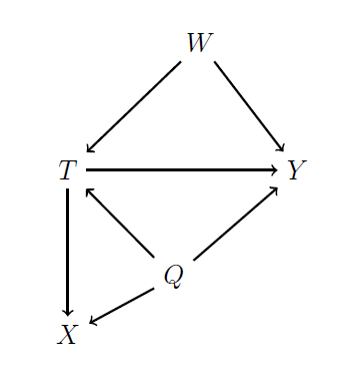
\includegraphics[width=0.4\textwidth,height=\textheight]{dag1.png}

\hfill\break

\textbf{Q1a} - Assume that you are interested in the relationship
between \(T\) and \(Y\) and that \(T\) only takes values of zero or one.
What would happen if you chose to estimate this relationship by
comparing the sample average of \(Y\) among observations where \(T=1\)
to the sample average of \(Y\) among observations where \(T=0\)?

\hfill\break
~~If you were to compare the observations of \(Y\) for the possible
values of \(T\) your\\
\hspace*{0.333em}\hspace*{0.333em}estimation would not represent the
affect of \(T\) on \(Y\). As the Directional Acyclic\\
\hspace*{0.333em}\hspace*{0.333em}Graph (DAG) above shows, both
variables \(Q\) and \(W\) influence the states of \(T\)\\
\hspace*{0.333em}\hspace*{0.333em}and \(Y\). Thus, without controlling
for those confounding variables the estimation\\
\hspace*{0.333em}\hspace*{0.333em}produced would not represent the true
relationship desired.

\hfill\break
\hfill\break

\textbf{Q1b} - Using conditional expectations, write out the ideal
comparison to identify the relationship between \(T\) and \(Y\).

\hfill\break
~~~The ideal comparison would look something like:\\
\hspace*{0.333em}\hspace*{0.333em}\hspace*{0.333em}\(E[Y|T=1,W=w,Q=q] - E[Y|T=0,W=w,Q=q]\)
for some constant \(w\) and \(q\).\\
\strut \\
\hspace*{0.333em}\hspace*{0.333em}\hspace*{0.333em}By holding the values
of the confounding variables constant we can then properly evaluate\\
\hspace*{0.333em}\hspace*{0.333em}\hspace*{0.333em}\(T\)'s influence on
\(Y\).

\hfill\break
\hfill\break

\hypertarget{q2---calculating-probabilities-with-known-distributions}{%
\section{Q2 - Calculating Probabilities with Known
Distributions}\label{q2---calculating-probabilities-with-known-distributions}}

\hfill\break

\textbf{Q2a} - Consider a random variable \(X\), where
\(X \sim N(0,1)\). Use R to find \(Pr(X \leq 1.64)\).

\hfill\break

\begin{Shaded}
\begin{Highlighting}[]
\CommentTok{\# Part (A)}
\CommentTok{\# Given x\textasciitilde{}N(0,1), where mean = 0 and var = 1, find Pr(X\textless{}=1.64)}
\NormalTok{meanA }\OtherTok{\textless{}{-}} \DecValTok{0}
\NormalTok{sdA }\OtherTok{\textless{}{-}} \FunctionTok{sqrt}\NormalTok{(}\DecValTok{1}\NormalTok{)}
\FunctionTok{pnorm}\NormalTok{(}\FloatTok{1.64}\NormalTok{,}\AttributeTok{mean=}\NormalTok{meanA,}\AttributeTok{sd=}\NormalTok{sdA,}\AttributeTok{lower.tail =}\NormalTok{ T)}
\end{Highlighting}
\end{Shaded}

\begin{verbatim}
## [1] 0.9494974
\end{verbatim}

\hfill\break

\textbf{Q2b} - Consider a random variable \(X\), where
\(X \sim N(42,8)\). Use R to find \(Pr(X \geq 30)\).

\hfill\break

\begin{Shaded}
\begin{Highlighting}[]
\CommentTok{\# Part (B)}
\CommentTok{\# Given X\textasciitilde{}N(42,8), where mean = 42 and var = 8, find Pr(X\textgreater{}=30)}
\NormalTok{meanB }\OtherTok{\textless{}{-}} \DecValTok{42}
\NormalTok{sdB }\OtherTok{\textless{}{-}} \FunctionTok{sqrt}\NormalTok{(}\DecValTok{8}\NormalTok{)}
\FunctionTok{pnorm}\NormalTok{(}\DecValTok{30}\NormalTok{,}\AttributeTok{mean=}\NormalTok{meanB,}\AttributeTok{sd=}\NormalTok{sdB,}\AttributeTok{lower.tail =}\NormalTok{ F)}
\end{Highlighting}
\end{Shaded}

\begin{verbatim}
## [1] 0.999989
\end{verbatim}

\hfill\break

\textbf{Q2c} - Consider a random variable \(X\), where
\(X \sim N(0,1)\). Use R to find \(Pr(|X| \geq 1.64)\).

\hfill\break

\begin{Shaded}
\begin{Highlighting}[]
\CommentTok{\# Part (C)}
\CommentTok{\# Given X\textasciitilde{}N(0,1), where mean = 0 and var = 1, find Pr(|X|\textgreater{}=1.64)}
\NormalTok{meanC }\OtherTok{\textless{}{-}} \DecValTok{0}
\NormalTok{sdC }\OtherTok{\textless{}{-}} \FunctionTok{sqrt}\NormalTok{(}\DecValTok{1}\NormalTok{)}
\NormalTok{upperC }\OtherTok{\textless{}{-}} \FunctionTok{pnorm}\NormalTok{(}\FloatTok{1.64}\NormalTok{,}\AttributeTok{mean=}\NormalTok{meanA,}\AttributeTok{sd=}\NormalTok{sdA,}\AttributeTok{lower.tail =}\NormalTok{ F)}
\NormalTok{lowerC }\OtherTok{\textless{}{-}} \FunctionTok{pnorm}\NormalTok{(}\SpecialCharTok{{-}}\FloatTok{1.64}\NormalTok{,}\AttributeTok{mean=}\NormalTok{meanA,}\AttributeTok{sd=}\NormalTok{sdA,}\AttributeTok{lower.tail =}\NormalTok{ T)}
\NormalTok{upperC }\SpecialCharTok{+}\NormalTok{ lowerC}
\end{Highlighting}
\end{Shaded}

\begin{verbatim}
## [1] 0.1010052
\end{verbatim}

\hfill\break

\textbf{Q2d} - Consider a random variable \(X\), where
\(X \sim N(0,1)\). Use R to find \(Pr(X \leq -1.64 \cup X \geq 2.5)\).

\hfill\break

\begin{Shaded}
\begin{Highlighting}[]
\CommentTok{\# Part (D)}
\CommentTok{\# Given X\textasciitilde{}N(0,1), where mean = 0 and var = 1, find Pr(X\textless{}={-}1.64 U X\textgreater{}=2.5)}
\NormalTok{meanD }\OtherTok{\textless{}{-}} \DecValTok{0}
\NormalTok{sdD }\OtherTok{\textless{}{-}} \FunctionTok{sqrt}\NormalTok{(}\DecValTok{1}\NormalTok{)}
\NormalTok{upperD }\OtherTok{\textless{}{-}} \FunctionTok{pnorm}\NormalTok{(}\FloatTok{2.5}\NormalTok{,}\AttributeTok{mean=}\NormalTok{meanA,}\AttributeTok{sd=}\NormalTok{sdA,}\AttributeTok{lower.tail =}\NormalTok{ F)}
\NormalTok{lowerD }\OtherTok{\textless{}{-}} \FunctionTok{pnorm}\NormalTok{(}\SpecialCharTok{{-}}\FloatTok{1.64}\NormalTok{,}\AttributeTok{mean=}\NormalTok{meanA,}\AttributeTok{sd=}\NormalTok{sdA,}\AttributeTok{lower.tail =}\NormalTok{ T)}
\NormalTok{upperD }\SpecialCharTok{+}\NormalTok{ lowerD}
\end{Highlighting}
\end{Shaded}

\begin{verbatim}
## [1] 0.05671225
\end{verbatim}

\hfill\break

\hypertarget{q3---the-age-of-umaine-students}{%
\section{Q3 - The Age of UMaine
Students}\label{q3---the-age-of-umaine-students}}

\textbf{Download the \texttt{E2data.RData} data set and load it in R.
Assume that the observations in the} \textit{universe} data frame
represent the entire population of UMaine students. Assume that the true
average age (\(\mu\)) of a UMaine student is 22.

\hfill\break

\textbf{Q3a} - Consider the three estimators proposed below. Show
whether each estimator is unbiased. Which one is the most efficient?**\\
\strut \\
For each of the below estimators, we will assume that an unbiased
estimator has an expected value that equals the population mean \(\mu\)

\begin{itemize}
\item
  \(\bar{y}= \frac{\sum_{i=1}^{n}{y_i}}{n}\)

  \begin{longtable}[]{@{}
    >{\raggedright\arraybackslash}p{(\columnwidth - 2\tabcolsep) * \real{0.5000}}
    >{\raggedright\arraybackslash}p{(\columnwidth - 2\tabcolsep) * \real{0.5000}}@{}}
  \toprule\noalign{}
  \begin{minipage}[b]{\linewidth}\raggedright
  Biasness
  \end{minipage} & \begin{minipage}[b]{\linewidth}\raggedright
  Efficiency
  \end{minipage} \\
  \midrule\noalign{}
  \endhead
  \bottomrule\noalign{}
  \endlastfoot
  \(\mu = E[\bar{y}]\) &
  \(var(\bar{y})=var(\frac{\sum_{i=1}^{n}{y_i}}{n})\) \\
  \(\mu = E[\frac{\sum_{i=1}^{n}{y_i}}{n}]\) &
  \(var(\bar{y})= (\frac{1}{n})^2 \cdot var(\sum_{i=1}^{n}{y_i})\) \\
  \(\mu = \frac{1}{n} \cdot E[\sum_{i=1}^{n}{y_i}]\) &
  \(var(\bar{y})= \frac{1}{n^2} \cdot \sum_{i=1}^{n}{var(y_i)}\) \\
  \(\mu = \frac{1}{n} \cdot \sum_{i=1}^{n}{E[y_i]}\) &
  \(var(\bar{y})= \frac{1}{n^2} \cdot n \cdot var(y_i)\) \\
  \(\mu = \frac{1}{n} \cdot \sum_{i=1}^{n}{\mu}\) &
  \(var(\bar{y})= \frac{n}{n^2} \cdot \sigma^2\) \\
  \(\mu = \frac{1}{n} \cdot n\mu\) &
  \(var(\bar{y})= \frac{\sigma^2}{n}\) \\
  \(\mu = \frac{n}{n} \cdot \mu\) & \\
  \(\mu = 1 \cdot \mu\) & \\
  \(\mu = \mu\) & \\
  \(\bar{y}\) is an unbiased estimator of \(\mu\) & \\
  \end{longtable}
\item
  \(\tilde{y}= \frac{\sum_{i=1}^{5}{y_i}}{5}\)

  \begin{longtable}[]{@{}
    >{\raggedright\arraybackslash}p{(\columnwidth - 2\tabcolsep) * \real{0.5000}}
    >{\raggedright\arraybackslash}p{(\columnwidth - 2\tabcolsep) * \real{0.5000}}@{}}
  \toprule\noalign{}
  \begin{minipage}[b]{\linewidth}\raggedright
  Biasness
  \end{minipage} & \begin{minipage}[b]{\linewidth}\raggedright
  Efficiency
  \end{minipage} \\
  \midrule\noalign{}
  \endhead
  \bottomrule\noalign{}
  \endlastfoot
  \(\mu = E[\tilde{y}]\) &
  \(var(\tilde{y})=var(\frac{\sum_{i=1}^{5}{y_i}}{5})\) \\
  \(\mu = E[\frac{\sum_{i=1}^{5}{y_i}}{5}]\) &
  \(var(\tilde{y})= (\frac{1}{5})^2 \cdot var(\sum_{i=1}^{5}{y_i})\) \\
  \(\mu = \frac{1}{5} \cdot E[\sum_{i=1}^{5}{y_i}]\) &
  \(var(\tilde{y})= \frac{1}{5^2} \cdot \sum_{i=1}^{5}{var(y_i)}\) \\
  \(\mu = \frac{1}{5} \cdot \sum_{i=1}^{5}{E[y_i]}\) &
  \(var(\tilde{y})= \frac{1}{5^2} \cdot 5 \cdot var(y_i)\) \\
  \(\mu = \frac{1}{5} \cdot \sum_{i=1}^{5}{\mu}\) &
  \(var(\tilde{y})= \frac{5}{5^2} \cdot \sigma^2\) \\
  \(\mu = \frac{1}{5} \cdot 5\mu\) &
  \(var(\tilde{y})= \frac{\sigma^2}{5}\) \\
  \(\mu = \frac{5}{5} \cdot \mu\) & \\
  \(\mu = 1 \cdot \mu\) & \\
  \(\mu = \mu\) & \\
  \(\tilde{y}\) is an unbiased estimator of \(\mu\) & \\
  \end{longtable}
\item
  \(\hat{y}=y_1\)

  \begin{longtable}[]{@{}
    >{\raggedright\arraybackslash}p{(\columnwidth - 2\tabcolsep) * \real{0.6338}}
    >{\raggedright\arraybackslash}p{(\columnwidth - 2\tabcolsep) * \real{0.3662}}@{}}
  \toprule\noalign{}
  \begin{minipage}[b]{\linewidth}\raggedright
  Biasness
  \end{minipage} & \begin{minipage}[b]{\linewidth}\raggedright
  Efficiency
  \end{minipage} \\
  \midrule\noalign{}
  \endhead
  \bottomrule\noalign{}
  \endlastfoot
  \(\mu = E[\hat{y}]\) & \(var(\hat{y})=var(y_i)\) \\
  \(\mu = E[y_1]\) & \(var(\hat{y})= \sigma^2\) \\
  \(\mu = \mu\) & \\
  \(\hat{y}\) is an unbiased estimator of \(\mu\) & \\
  \end{longtable}
\end{itemize}

\hfill\break
Given that estimators with smaller variances are more efficient,
\(\hat{y}\) is the least efficient estimator with
\(var(\hat{y})= \sigma^2\). The most efficient estimator is \(\bar{y}\)
for samples greater than 5 observations
(\(var(\bar{y})= \frac{\sigma^2}{n}\)). For samples with less than 5
observations, \(\tilde{y}\) is the most efficient
(\(var(\bar{y})= \frac{\sigma^2}{n}\)). Thus:

\begin{longtable}[]{@{}cc@{}}
\toprule\noalign{}
Sample Size & Efficiency Ranking \\
\midrule\noalign{}
\endhead
\bottomrule\noalign{}
\endlastfoot
\(n < 5\) & \(\bar{y} > \tilde{y} > \hat{y}\) \\
\(n = 5\) & \(\bar{y} = \tilde{y} > \hat{y}\) \\
\(n > 5\) & \(\tilde{y} > \bar{y} > \hat{y}\) \\
\end{longtable}

\hfill\break
\hfill\break

\textbf{Q3b} - Draw a sample of 25 observations from the
\textit{universe} data frame. Using the sample, calculate an estimate of
\(\mu\) using \(\bar{y}\), \(\tilde{y}\) and \(\hat{y}\). Report your
estimates. Which one is the closest to the true value of \(\mu\)?\\

\begin{Shaded}
\begin{Highlighting}[]
\CommentTok{\# Sets working directory to data folder for Exercise 2}
\FunctionTok{setwd}\NormalTok{(datapath)}
\CommentTok{\# Loads RData file for the assignment}
\FunctionTok{load}\NormalTok{(}\AttributeTok{file=}\StringTok{"E2data.RDATA"}\NormalTok{)}

\CommentTok{\# Sets the sample size and mean (mu) for later use}
\NormalTok{sample.size }\OtherTok{\textless{}{-}} \DecValTok{25}
\NormalTok{mu }\OtherTok{\textless{}{-}} \DecValTok{22}
\CommentTok{\# Sets a seed for later review}
\FunctionTok{set.seed}\NormalTok{(}\AttributeTok{seed=}\DecValTok{8675309}\NormalTok{)}

\CommentTok{\# Takes a sample of size sample.size from the universe data frame and stores the values in }
\CommentTok{\# the universe.sample data frame}
\NormalTok{universe.sample }\OtherTok{\textless{}{-}} \FunctionTok{sample\_n}\NormalTok{(universe,}\AttributeTok{size =}\NormalTok{ sample.size,}\AttributeTok{replace=}\NormalTok{F)}

\CommentTok{\# Calculates the values of the y\_bar, y\_tilde, and y\_hat estimators}
\NormalTok{y\_bar }\OtherTok{\textless{}{-}} \FunctionTok{sum}\NormalTok{(universe.sample}\SpecialCharTok{$}\NormalTok{age)}\SpecialCharTok{/}\NormalTok{sample.size}
\NormalTok{y\_tilde }\OtherTok{\textless{}{-}} \FunctionTok{sum}\NormalTok{(universe.sample[}\DecValTok{1}\SpecialCharTok{:}\DecValTok{5}\NormalTok{,}\DecValTok{1}\NormalTok{])}\SpecialCharTok{/}\DecValTok{5}
\NormalTok{y\_hat }\OtherTok{\textless{}{-}}\NormalTok{ universe.sample[}\DecValTok{1}\NormalTok{,}\DecValTok{1}\NormalTok{]}

\CommentTok{\# Determines the distance (in absolute value terms) of each estimator from the population mean}
\NormalTok{mu\_y\_bar }\OtherTok{\textless{}{-}} \FunctionTok{abs}\NormalTok{(y\_bar }\SpecialCharTok{{-}}\NormalTok{ mu)}
\NormalTok{mu\_y\_tilde }\OtherTok{\textless{}{-}} \FunctionTok{abs}\NormalTok{(y\_tilde }\SpecialCharTok{{-}}\NormalTok{ mu)}
\NormalTok{mu\_y\_hat }\OtherTok{\textless{}{-}}  \FunctionTok{abs}\NormalTok{(y\_hat }\SpecialCharTok{{-}}\NormalTok{ mu)}

\CommentTok{\# Determines which of the above differences is least}
\NormalTok{smallest\_difference }\OtherTok{\textless{}{-}} \FunctionTok{min}\NormalTok{(}\FunctionTok{c}\NormalTok{(mu\_y\_bar,mu\_y\_tilde,mu\_y\_hat))}

\CommentTok{\# Reports the estimator that is closest to the population mean and then reports that}
\CommentTok{\# difference in numerical terms. }
\ControlFlowTok{if}\NormalTok{(smallest\_difference }\SpecialCharTok{==}\NormalTok{ mu\_y\_bar)\{}\FunctionTok{print}\NormalTok{(}\StringTok{"y\_bar is the closest estimator to the mean mu = 22"}\NormalTok{)\}}
\end{Highlighting}
\end{Shaded}

\begin{verbatim}
## [1] "y_bar is the closest estimator to the mean mu = 22"
\end{verbatim}

\begin{Shaded}
\begin{Highlighting}[]
\ControlFlowTok{if}\NormalTok{(smallest\_difference }\SpecialCharTok{==}\NormalTok{ mu\_y\_tilde)\{}\FunctionTok{print}\NormalTok{(}\StringTok{"y\_tilde is the closest estimator to the mean mu = 22"}\NormalTok{)\}}
\ControlFlowTok{if}\NormalTok{(smallest\_difference }\SpecialCharTok{==}\NormalTok{ mu\_y\_hat)\{}\FunctionTok{print}\NormalTok{(}\StringTok{"y\_hat is the closest estimator to the mean mu = 22"}\NormalTok{)\}}
\FunctionTok{print}\NormalTok{(smallest\_difference)}
\end{Highlighting}
\end{Shaded}

\begin{verbatim}
## [1] 0.3725899
\end{verbatim}

\hfill\break
\hfill\break

\hypertarget{q4---hypothesis-testing}{%
\section{Q4 - Hypothesis Testing}\label{q4---hypothesis-testing}}

\textbf{Imagine that you are interested the effect of going on a daily
jog (}\(\hat{\beta}\)) and life expectancy.

\begin{itemize}
\item
  \textbf{You estimate} \(\hat{\beta} = 6.25\) after analyzing a sample
  of 502 observations.
\item
  \textbf{The standard error of your estimate is 1.43.}
\end{itemize}

\hfill\break

\textbf{Q4a} - Test the following null hypotheses against the
alternative, assuming you are willing to accept a 5\% chance of
committing a Type I error:**

\hfill\break

\begin{itemize}
\item
  \(H_0: \: \beta=9.25\)
\item
  \(H_0: \: \beta=2.1\)
\item
  \(H_0: \: \beta=3.5\)
\end{itemize}

\begin{Shaded}
\begin{Highlighting}[]
\CommentTok{\# Part (a)}
\CommentTok{\# Declare variables for our estimated beta (\textquotesingle{}beta\_hat\textquotesingle{}), number of observations }
\CommentTok{\# (n, stored as \textquotesingle{}obs\textquotesingle{}), and the standard error of our estimate \textquotesingle{}se\textquotesingle{}}
\NormalTok{beta\_hat }\OtherTok{\textless{}{-}} \FloatTok{6.25}
\NormalTok{obs }\OtherTok{\textless{}{-}} \DecValTok{502}
\NormalTok{se }\OtherTok{\textless{}{-}} \FloatTok{1.43}

\CommentTok{\# Declares the acceptable bound for one tail of the distribution}
\NormalTok{bound }\OtherTok{\textless{}{-}} \FloatTok{0.025}

\CommentTok{\# Declare the null hypothesis values for tests 1, 2, and 3}
\NormalTok{hyp\_1 }\OtherTok{\textless{}{-}} \FloatTok{9.25}
\NormalTok{hyp\_2 }\OtherTok{\textless{}{-}} \FloatTok{2.1}
\NormalTok{hyp\_3 }\OtherTok{\textless{}{-}} \FloatTok{3.5}

\CommentTok{\# Determines the proportion of the distribution that resides above each hypothesis}
\NormalTok{upper\_1 }\OtherTok{\textless{}{-}} \FunctionTok{pnorm}\NormalTok{(hyp\_1,}\AttributeTok{mean=}\NormalTok{beta\_hat,}\AttributeTok{sd=}\NormalTok{se,}\AttributeTok{lower.tail =}\NormalTok{ F)}
\NormalTok{upper\_2 }\OtherTok{\textless{}{-}} \FunctionTok{pnorm}\NormalTok{(hyp\_2,}\AttributeTok{mean=}\NormalTok{beta\_hat,}\AttributeTok{sd=}\NormalTok{se,}\AttributeTok{lower.tail =}\NormalTok{ F)}
\NormalTok{upper\_3 }\OtherTok{\textless{}{-}} \FunctionTok{pnorm}\NormalTok{(hyp\_3,}\AttributeTok{mean=}\NormalTok{beta\_hat,}\AttributeTok{sd=}\NormalTok{se,}\AttributeTok{lower.tail =}\NormalTok{ F)}
\CommentTok{\# Determines the proportion of the distribution that resides below each hypothesis}
\NormalTok{lower\_1 }\OtherTok{\textless{}{-}} \FunctionTok{pnorm}\NormalTok{(hyp\_1,}\AttributeTok{mean=}\NormalTok{beta\_hat,}\AttributeTok{sd=}\NormalTok{se,}\AttributeTok{lower.tail =}\NormalTok{ T)}
\NormalTok{lower\_2 }\OtherTok{\textless{}{-}} \FunctionTok{pnorm}\NormalTok{(hyp\_2,}\AttributeTok{mean=}\NormalTok{beta\_hat,}\AttributeTok{sd=}\NormalTok{se,}\AttributeTok{lower.tail =}\NormalTok{ T)}
\NormalTok{lower\_3 }\OtherTok{\textless{}{-}} \FunctionTok{pnorm}\NormalTok{(hyp\_3,}\AttributeTok{mean=}\NormalTok{beta\_hat,}\AttributeTok{sd=}\NormalTok{se,}\AttributeTok{lower.tail =}\NormalTok{ T)}

\CommentTok{\# Creates a boolean value to determine if each hypothesis is within the 5\% unallowed}
\CommentTok{\# portion of the distribution. }
\NormalTok{hyp\_test\_1 }\OtherTok{\textless{}{-}}\NormalTok{ (upper\_1 }\SpecialCharTok{\textgreater{}}\NormalTok{ bound }\SpecialCharTok{\&}\NormalTok{ lower\_1 }\SpecialCharTok{\textgreater{}}\NormalTok{ bound)}
\NormalTok{hyp\_test\_2 }\OtherTok{\textless{}{-}}\NormalTok{ (upper\_2 }\SpecialCharTok{\textgreater{}}\NormalTok{ bound }\SpecialCharTok{\&}\NormalTok{ lower\_2 }\SpecialCharTok{\textgreater{}}\NormalTok{ bound)}
\NormalTok{hyp\_test\_3 }\OtherTok{\textless{}{-}}\NormalTok{ (upper\_3 }\SpecialCharTok{\textgreater{}}\NormalTok{ bound }\SpecialCharTok{\&}\NormalTok{ lower\_3 }\SpecialCharTok{\textgreater{}}\NormalTok{ bound)}

\CommentTok{\# Reports to the console the results of the above tests in plain language}
\FunctionTok{paste}\NormalTok{(}\StringTok{"For hypothesis 1 of beta ="}\NormalTok{,hyp\_1,}\StringTok{"we cannot reject the hypothesis {-} TRUE or FALSE?"}\NormalTok{,hyp\_test\_1,}\AttributeTok{sep=}\StringTok{" "}\NormalTok{)}
\end{Highlighting}
\end{Shaded}

\begin{verbatim}
## [1] "For hypothesis 1 of beta = 9.25 we cannot reject the hypothesis - TRUE or FALSE? FALSE"
\end{verbatim}

\begin{Shaded}
\begin{Highlighting}[]
\FunctionTok{paste}\NormalTok{(}\StringTok{"For hypothesis 2 of beta ="}\NormalTok{,hyp\_2,}\StringTok{"we cannot reject the hypothesis {-} TRUE or FALSE?"}\NormalTok{,hyp\_test\_2,}\AttributeTok{sep=}\StringTok{" "}\NormalTok{)}
\end{Highlighting}
\end{Shaded}

\begin{verbatim}
## [1] "For hypothesis 2 of beta = 2.1 we cannot reject the hypothesis - TRUE or FALSE? FALSE"
\end{verbatim}

\begin{Shaded}
\begin{Highlighting}[]
\FunctionTok{paste}\NormalTok{(}\StringTok{"For hypothesis 3 of beta ="}\NormalTok{,hyp\_3,}\StringTok{"we cannot reject the hypothesis {-} TRUE or FALSE?"}\NormalTok{,hyp\_test\_3,}\AttributeTok{sep=}\StringTok{" "}\NormalTok{)}
\end{Highlighting}
\end{Shaded}

\begin{verbatim}
## [1] "For hypothesis 3 of beta = 3.5 we cannot reject the hypothesis - TRUE or FALSE? TRUE"
\end{verbatim}

\hfill\break
\hfill\break

\textbf{Q4b} - Still using the estimate from above, construct the
following confidence intervals. Plot the confidence intervals in R and
be sure to interpret each interval in words.

\hfill\break

\begin{Shaded}
\begin{Highlighting}[]
\CommentTok{\# Part (b)}
\CommentTok{\# Determines the upper bounds for a 95\% and 99\% CI for mean = beta\_hat, standard}
\CommentTok{\# deviation = se (our standard error variable)}
\NormalTok{upper\_95 }\OtherTok{\textless{}{-}} \FunctionTok{round}\NormalTok{(}\FunctionTok{qnorm}\NormalTok{(}\FloatTok{0.975}\NormalTok{,}\AttributeTok{mean=}\NormalTok{beta\_hat,}\AttributeTok{sd=}\NormalTok{se,}\AttributeTok{lower.tail =}\NormalTok{ T),}\AttributeTok{digits =} \DecValTok{2}\NormalTok{)}
\NormalTok{upper\_99 }\OtherTok{\textless{}{-}} \FunctionTok{round}\NormalTok{(}\FunctionTok{qnorm}\NormalTok{(}\FloatTok{0.995}\NormalTok{,}\AttributeTok{mean=}\NormalTok{beta\_hat,}\AttributeTok{sd=}\NormalTok{se,}\AttributeTok{lower.tail =}\NormalTok{ T),}\AttributeTok{digits =} \DecValTok{2}\NormalTok{)}

\CommentTok{\# Determines the lower bounds for a 95\% and 99\% CI for mean = beta\_hat, standard}
\CommentTok{\# deviation = se (our standard error variable)}
\NormalTok{lower\_95 }\OtherTok{\textless{}{-}} \FunctionTok{round}\NormalTok{(}\FunctionTok{qnorm}\NormalTok{(}\FloatTok{0.025}\NormalTok{,}\AttributeTok{mean=}\NormalTok{beta\_hat,}\AttributeTok{sd=}\NormalTok{se,}\AttributeTok{lower.tail =}\NormalTok{ T),}\AttributeTok{digits =} \DecValTok{2}\NormalTok{)}
\NormalTok{lower\_99 }\OtherTok{\textless{}{-}} \FunctionTok{round}\NormalTok{(}\FunctionTok{qnorm}\NormalTok{(}\FloatTok{0.005}\NormalTok{,}\AttributeTok{mean=}\NormalTok{beta\_hat,}\AttributeTok{sd=}\NormalTok{se,}\AttributeTok{lower.tail =}\NormalTok{ T),}\AttributeTok{digits =} \DecValTok{2}\NormalTok{)}

\CommentTok{\# Stores the upper and lower bounds of the 95\% CI in the vector \textquotesingle{}conf\_95\textquotesingle{} and prints}
\CommentTok{\# the values to the console}
\NormalTok{conf\_95 }\OtherTok{\textless{}{-}} \FunctionTok{c}\NormalTok{(lower\_95,upper\_95)}
\NormalTok{conf\_95}
\end{Highlighting}
\end{Shaded}

\begin{verbatim}
## [1] 3.45 9.05
\end{verbatim}

\begin{Shaded}
\begin{Highlighting}[]
\CommentTok{\# Stores the upper and lower bounds of the 99\% CI in the vector \textquotesingle{}conf\_99\textquotesingle{} and prints}
\CommentTok{\# the values to the console}
\NormalTok{conf\_99 }\OtherTok{\textless{}{-}} \FunctionTok{c}\NormalTok{(lower\_99,upper\_99)}
\NormalTok{conf\_99}
\end{Highlighting}
\end{Shaded}

\begin{verbatim}
## [1] 2.57 9.93
\end{verbatim}

\hfill\break
The above confidence intervals represent the set of values we would
reject/fail to reject a hypothesis givena Type I error tolerance of 95\%
and 99\%, respectively\\
\strut \\

\textbf{Q4c} - What is the smallest sized test for which you would
reject the null hypotheses \(H_0: \: \beta=4\)\\

\begin{Shaded}
\begin{Highlighting}[]
\CommentTok{\# Part (c)}
\CommentTok{\# Declares the hypothesis that beta = 4 for testing. Stores value in \textquotesingle{}hyp\_c\textquotesingle{}}
\NormalTok{hyp\_c }\OtherTok{\textless{}{-}} \DecValTok{4}

\CommentTok{\# Determines the proportion of the distribution above and below the hyp\_c value}
\NormalTok{below\_c }\OtherTok{\textless{}{-}} \FunctionTok{round}\NormalTok{(}\FunctionTok{pnorm}\NormalTok{(hyp\_c,}\AttributeTok{mean=}\NormalTok{beta\_hat,}\AttributeTok{sd=}\NormalTok{se,}\AttributeTok{lower.tail =}\NormalTok{ T),}\AttributeTok{digits =} \DecValTok{2}\NormalTok{)}
\NormalTok{above\_c }\OtherTok{\textless{}{-}} \FunctionTok{round}\NormalTok{(}\FunctionTok{pnorm}\NormalTok{(hyp\_c,}\AttributeTok{mean=}\NormalTok{beta\_hat,}\AttributeTok{sd=}\NormalTok{se,}\AttributeTok{lower.tail =}\NormalTok{ F),}\AttributeTok{digits =} \DecValTok{2}\NormalTok{)}

\CommentTok{\# Determines the lesser of the above proportions and takes that as the one{-}tail alpha.}
\CommentTok{\# Then multiplies that value by two for a two tail test for reporting to the user. }
\NormalTok{alpha\_c }\OtherTok{\textless{}{-}} \DecValTok{2}\SpecialCharTok{*}\FunctionTok{min}\NormalTok{(}\FunctionTok{c}\NormalTok{(below\_c,above\_c))}

\CommentTok{\# Displays results in console using natural language.}
\FunctionTok{paste}\NormalTok{(}\StringTok{"For the hypothesis beta ="}\NormalTok{,hyp\_c,}\StringTok{" we would reject the hypothesis if using an alpha value of"}\NormalTok{,alpha\_c,}\AttributeTok{sep=}\StringTok{" "}\NormalTok{)}
\end{Highlighting}
\end{Shaded}

\begin{verbatim}
## [1] "For the hypothesis beta = 4  we would reject the hypothesis if using an alpha value of 0.12"
\end{verbatim}

\hfill\break
\hfill\break

\hypertarget{q5---the-effect-of-studying-hard-on-gpa}{%
\section{Q5 - The Effect of Studying Hard on
GPA}\label{q5---the-effect-of-studying-hard-on-gpa}}

\hfill\break

\textbf{Q5a} - Using the full sample, calculate an estimate of
\(\hat{\gamma}\).\\

\begin{Shaded}
\begin{Highlighting}[]
\CommentTok{\# Part (a)}
\CommentTok{\# This bit of code just proves that there are no values above 1 or below 0 for the}
\CommentTok{\# study.hard column of the universe data frame. Understanding this aspect of the data}
\CommentTok{\# will be important for the approach I take later. }
\FunctionTok{max}\NormalTok{(universe}\SpecialCharTok{$}\NormalTok{study.hard)}
\end{Highlighting}
\end{Shaded}

\begin{verbatim}
## [1] 1
\end{verbatim}

\begin{Shaded}
\begin{Highlighting}[]
\FunctionTok{min}\NormalTok{(universe}\SpecialCharTok{$}\NormalTok{study.hard)}
\end{Highlighting}
\end{Shaded}

\begin{verbatim}
## [1] 0
\end{verbatim}

\begin{Shaded}
\begin{Highlighting}[]
\CommentTok{\# Takes the mean of GPAs in the full sample where case (0) is study.hard = 0 and}
\CommentTok{\# where case (1) is study.hard = 1. Stores the conditional means in y0\_bar for case (0)}
\CommentTok{\# and y1\_bar for case (1)}
\NormalTok{y0\_bar }\OtherTok{\textless{}{-}} \FunctionTok{mean}\NormalTok{(universe}\SpecialCharTok{$}\NormalTok{gpa[universe}\SpecialCharTok{$}\NormalTok{study.hard}\SpecialCharTok{==}\DecValTok{0}\NormalTok{])}
\NormalTok{y1\_bar }\OtherTok{\textless{}{-}} \FunctionTok{mean}\NormalTok{(universe}\SpecialCharTok{$}\NormalTok{gpa[universe}\SpecialCharTok{$}\NormalTok{study.hard}\SpecialCharTok{==}\DecValTok{1}\NormalTok{])}

\CommentTok{\# Takes the sum of all GPA\textquotesingle{}s divided by themselves to create a count of observations}
\CommentTok{\# then subtracts the count of observations where study.hard =/= 0}
\NormalTok{n0 }\OtherTok{\textless{}{-}} \FunctionTok{sum}\NormalTok{(universe}\SpecialCharTok{$}\NormalTok{gpa}\SpecialCharTok{/}\NormalTok{universe}\SpecialCharTok{$}\NormalTok{gpa)}\SpecialCharTok{{-}}\FunctionTok{sum}\NormalTok{(universe}\SpecialCharTok{$}\NormalTok{study.hard)}
\CommentTok{\# Sums all of the values of study.hard where study.hard =/= 0 }
\NormalTok{n1 }\OtherTok{\textless{}{-}} \FunctionTok{sum}\NormalTok{(universe}\SpecialCharTok{$}\NormalTok{study.hard)}

\CommentTok{\# Calculates the sample variance for case (0) (stored as S0\_2) and case (1) (stored}
\CommentTok{\# as s1\_2).}
\NormalTok{s0\_2 }\OtherTok{\textless{}{-}} \FunctionTok{var}\NormalTok{(universe}\SpecialCharTok{$}\NormalTok{gpa[universe}\SpecialCharTok{$}\NormalTok{study.hard}\SpecialCharTok{==}\DecValTok{0}\NormalTok{])}
\NormalTok{s1\_2 }\OtherTok{\textless{}{-}} \FunctionTok{var}\NormalTok{(universe}\SpecialCharTok{$}\NormalTok{gpa[universe}\SpecialCharTok{$}\NormalTok{study.hard}\SpecialCharTok{==}\DecValTok{1}\NormalTok{])}

\CommentTok{\# Calculates gamma\_hat based on the values of y0\_bar and y1\_bar and reports to the console}
\NormalTok{gamma\_hat }\OtherTok{\textless{}{-}}\NormalTok{ y1\_bar }\SpecialCharTok{{-}}\NormalTok{ y0\_bar}
\NormalTok{gamma\_hat}
\end{Highlighting}
\end{Shaded}

\begin{verbatim}
## [1] 1.254598
\end{verbatim}

\hfill\break
\hfill\break

\textbf{Q5b} - Calculate the standard error associated with your
estimate.\\

\begin{Shaded}
\begin{Highlighting}[]
\CommentTok{\# Part (b)}
\CommentTok{\# Using the above calculated s0\_2, s1\_2, n0, and n1 we can determine the standard}
\CommentTok{\# error for gamma\_hat}
\NormalTok{se }\OtherTok{\textless{}{-}} \FunctionTok{sqrt}\NormalTok{((s1\_2}\SpecialCharTok{/}\NormalTok{n1)}\SpecialCharTok{+}\NormalTok{(s0\_2}\SpecialCharTok{/}\NormalTok{n0))}
\NormalTok{se}
\end{Highlighting}
\end{Shaded}

\begin{verbatim}
## [1] 0.02186911
\end{verbatim}

\hfill\break
\hfill\break

\textbf{Q5c} - Test the hypothesis that studying hard has no effect on
GPA\\
In order to determine if there is a GPA effect due to studying hard, we
will assume that there is NO GPA effect due to studying hard
(\(H_0: \hat{\gamma} = 0\)). If this is true, than we would expect that,
on average, \(\hat{\gamma} = 0\). We will test to see if our observed
gamma\_hat is outside of values of alpha associated with a 95\% CI. This
means that an upper\_gamma value less than 0.025 or a lower value less
than 0.025 would cause us to reject the hypothesis
\(H_0: \hat{\gamma} = 0\).\\

\begin{Shaded}
\begin{Highlighting}[]
\CommentTok{\# Part (c)}
\CommentTok{\# Declare alpha}
\NormalTok{alpha }\OtherTok{=} \FloatTok{0.025}
\CommentTok{\# Determine the proportion of the distribution that is higher than our observed}
\CommentTok{\# gamma\_hat}
\NormalTok{upper\_gamma }\OtherTok{\textless{}{-}} \FunctionTok{pnorm}\NormalTok{(gamma\_hat,}\AttributeTok{mean =} \DecValTok{0}\NormalTok{, }\AttributeTok{sd=}\NormalTok{se,}\AttributeTok{lower.tail =}\NormalTok{ F)}
\NormalTok{upper\_gamma}
\end{Highlighting}
\end{Shaded}

\begin{verbatim}
## [1] 0
\end{verbatim}

\begin{Shaded}
\begin{Highlighting}[]
\CommentTok{\# Determine the proportion of the distribution that is lower than our observed}
\CommentTok{\# gamma\_hat}
\NormalTok{lower\_gamma }\OtherTok{\textless{}{-}} \FunctionTok{pnorm}\NormalTok{(gamma\_hat,}\AttributeTok{mean =} \DecValTok{0}\NormalTok{, }\AttributeTok{sd=}\NormalTok{se, }\AttributeTok{lower.tail=}\NormalTok{T)}
\NormalTok{lower\_gamma}
\end{Highlighting}
\end{Shaded}

\begin{verbatim}
## [1] 1
\end{verbatim}

\begin{Shaded}
\begin{Highlighting}[]
\CommentTok{\# Since the value of upper\_gamma is 0, we can reject the hypothesis that gamma\_hat = 0}
\NormalTok{gamma\_hyp\_test }\OtherTok{\textless{}{-}}\NormalTok{ ((upper\_gamma }\SpecialCharTok{\textless{}}\NormalTok{ alpha)}\SpecialCharTok{|}\NormalTok{(lower\_gamma }\SpecialCharTok{\textless{}}\NormalTok{ alpha))}
\FunctionTok{paste}\NormalTok{(}\StringTok{"For hypothesis of gamma\_hat = 0, we reject the hypothesis {-} TRUE or FALSE?"}\NormalTok{,gamma\_hyp\_test,}\AttributeTok{sep=}\StringTok{" "}\NormalTok{)}
\end{Highlighting}
\end{Shaded}

\begin{verbatim}
## [1] "For hypothesis of gamma_hat = 0, we reject the hypothesis - TRUE or FALSE? TRUE"
\end{verbatim}

\hfill\break
\hfill\break

\textbf{Q5d} - Construct and discuss a 95 \% confidence interval around
your estimate of \(\hat{\gamma}\)\\

\begin{Shaded}
\begin{Highlighting}[]
\CommentTok{\# Part (d)}
\CommentTok{\# First, we will create the upper and lower bounds of the 95\% CI using the qnorm}
\CommentTok{\# function measured from the lower tail of the distribution}
\NormalTok{gamma\_95u }\OtherTok{\textless{}{-}} \FunctionTok{round}\NormalTok{(}\FunctionTok{qnorm}\NormalTok{(}\FloatTok{0.975}\NormalTok{,}\AttributeTok{mean =}\NormalTok{ gamma\_hat,}\AttributeTok{sd=}\NormalTok{se,}\AttributeTok{lower.tail =}\NormalTok{ T),}\AttributeTok{digits=}\DecValTok{2}\NormalTok{)}
\NormalTok{gamma\_95l }\OtherTok{\textless{}{-}} \FunctionTok{round}\NormalTok{(}\FunctionTok{qnorm}\NormalTok{(}\FloatTok{0.025}\NormalTok{,}\AttributeTok{mean =}\NormalTok{ gamma\_hat,}\AttributeTok{sd=}\NormalTok{se,}\AttributeTok{lower.tail=}\NormalTok{T),}\AttributeTok{digits=}\DecValTok{2}\NormalTok{)}

\CommentTok{\# We place the lower and upper bounds of the 95\% CI a vector named \textquotesingle{}gamma\_95CI\textquotesingle{} for}
\CommentTok{\# reporting to the console}
\NormalTok{gamma\_95CI }\OtherTok{\textless{}{-}} \FunctionTok{c}\NormalTok{(gamma\_95l,gamma\_95u)}
\NormalTok{gamma\_95CI}
\end{Highlighting}
\end{Shaded}

\begin{verbatim}
## [1] 1.21 1.30
\end{verbatim}

\hfill\break

This confidence interval represents the values of \(\hat{\gamma}\) for
which we would reject or fail to reject a hypothesis given
\(\alpha = 0.05\).\\
\strut \\

\hypertarget{q6conditional-on-the-library}{%
\section{\texorpdfstring{\textbf{Q6\ldots Conditional on the
library}}{Q6\ldots Conditional on the library}}\label{q6conditional-on-the-library}}

Repeat the tasks from Q5a, Q5b, and Q5d, but this time focus only on
students who know where the library is. Compare and contrast your
results to those you obtained in Q5.\\
\strut \\
\textbf{Q6a} - Using the full sample, calculate an estimate of
\(\hat{\gamma}\) conditioned on knowing where the library is.\\

\begin{Shaded}
\begin{Highlighting}[]
\CommentTok{\# Part (a)}
\CommentTok{\# This code is reused from (5a), but with a term added to condition the estimators}
\CommentTok{\# on students knowing where the library is (library = 1)}
\FunctionTok{max}\NormalTok{(universe}\SpecialCharTok{$}\NormalTok{library)}
\end{Highlighting}
\end{Shaded}

\begin{verbatim}
## [1] 1
\end{verbatim}

\begin{Shaded}
\begin{Highlighting}[]
\FunctionTok{min}\NormalTok{(universe}\SpecialCharTok{$}\NormalTok{library)}
\end{Highlighting}
\end{Shaded}

\begin{verbatim}
## [1] 0
\end{verbatim}

\begin{Shaded}
\begin{Highlighting}[]
\CommentTok{\# Takes the mean of GPAs in the full sample where case (0) is study.hard = 0 and}
\CommentTok{\# where case (1) is study.hard = 1. Stores the conditional means in y0\_bar for case (0)}
\CommentTok{\# and y1\_bar for case (1)}
\NormalTok{y0\_bar6 }\OtherTok{\textless{}{-}} \FunctionTok{mean}\NormalTok{(universe}\SpecialCharTok{$}\NormalTok{gpa[universe}\SpecialCharTok{$}\NormalTok{study.hard}\SpecialCharTok{==}\DecValTok{0} \SpecialCharTok{\&}\NormalTok{ universe}\SpecialCharTok{$}\NormalTok{library}\SpecialCharTok{==}\DecValTok{1}\NormalTok{])}
\NormalTok{y1\_bar6 }\OtherTok{\textless{}{-}} \FunctionTok{mean}\NormalTok{(universe}\SpecialCharTok{$}\NormalTok{gpa[universe}\SpecialCharTok{$}\NormalTok{study.hard}\SpecialCharTok{==}\DecValTok{1} \SpecialCharTok{\&}\NormalTok{ universe}\SpecialCharTok{$}\NormalTok{library}\SpecialCharTok{==}\DecValTok{1}\NormalTok{])}

\CommentTok{\# Takes the sum of all GPA\textquotesingle{}s divided by themselves to create a count of observations}
\CommentTok{\# then subtracts the count of observations where study.hard =/= 0}
\NormalTok{n06 }\OtherTok{\textless{}{-}} \FunctionTok{sum}\NormalTok{(universe}\SpecialCharTok{$}\NormalTok{gpa[universe}\SpecialCharTok{$}\NormalTok{library}\SpecialCharTok{==}\DecValTok{1}\NormalTok{]}\SpecialCharTok{/}\NormalTok{universe}\SpecialCharTok{$}\NormalTok{gpa[universe}\SpecialCharTok{$}\NormalTok{library}\SpecialCharTok{==}\DecValTok{1}\NormalTok{])}\SpecialCharTok{{-}}\FunctionTok{sum}\NormalTok{(universe}\SpecialCharTok{$}\NormalTok{study.hard[universe}\SpecialCharTok{$}\NormalTok{library}\SpecialCharTok{==}\DecValTok{1}\NormalTok{])}
\CommentTok{\# Sums all of the values of study.hard where study.hard =/= 0 }
\NormalTok{n16 }\OtherTok{\textless{}{-}} \FunctionTok{sum}\NormalTok{(universe}\SpecialCharTok{$}\NormalTok{study.hard[universe}\SpecialCharTok{$}\NormalTok{library}\SpecialCharTok{==}\DecValTok{1}\NormalTok{])}

\CommentTok{\# Calculates the sample variance for case (0) (stored as S0\_2) and case (1) (stored}
\CommentTok{\# as s1\_2).}
\NormalTok{s0\_26 }\OtherTok{\textless{}{-}} \FunctionTok{var}\NormalTok{(universe}\SpecialCharTok{$}\NormalTok{gpa[universe}\SpecialCharTok{$}\NormalTok{study.hard}\SpecialCharTok{==}\DecValTok{0} \SpecialCharTok{\&}\NormalTok{ universe}\SpecialCharTok{$}\NormalTok{library}\SpecialCharTok{==}\DecValTok{1}\NormalTok{])}
\NormalTok{s1\_26 }\OtherTok{\textless{}{-}} \FunctionTok{var}\NormalTok{(universe}\SpecialCharTok{$}\NormalTok{gpa[universe}\SpecialCharTok{$}\NormalTok{study.hard}\SpecialCharTok{==}\DecValTok{1} \SpecialCharTok{\&}\NormalTok{ universe}\SpecialCharTok{$}\NormalTok{library}\SpecialCharTok{==}\DecValTok{1}\NormalTok{])}

\CommentTok{\# Calculates gamma\_hat based on the values of y0\_bar and y1\_bar and reports to the console}
\NormalTok{gamma\_hat6 }\OtherTok{\textless{}{-}}\NormalTok{ y1\_bar6 }\SpecialCharTok{{-}}\NormalTok{ y0\_bar6}
\NormalTok{gamma\_hat6}
\end{Highlighting}
\end{Shaded}

\begin{verbatim}
## [1] 0.9625202
\end{verbatim}

\hfill\break
\hfill\break
\textbf{Q6b} - Calculate the standard error associated with your
estimate conditioned on knowing where the library is.\\

\begin{Shaded}
\begin{Highlighting}[]
\CommentTok{\# Part (b)}
\CommentTok{\# Again, code is reused from (5b)}
\CommentTok{\# Using the above calculated s0\_2, s1\_2, n0, and n1 we can determine the standard}
\CommentTok{\# error for gamma\_hat}
\NormalTok{se6 }\OtherTok{\textless{}{-}} \FunctionTok{sqrt}\NormalTok{((s1\_26}\SpecialCharTok{/}\NormalTok{n16)}\SpecialCharTok{+}\NormalTok{(s0\_26}\SpecialCharTok{/}\NormalTok{n06))}
\NormalTok{se6}
\end{Highlighting}
\end{Shaded}

\begin{verbatim}
## [1] 0.03841955
\end{verbatim}

\hfill\break
\hfill\break
\textbf{Q6d} - Construct and discuss a 95 \% confidence interval around
your estimate of \(\hat{\gamma}\) conditioned on knowing where the
library is\\

\begin{Shaded}
\begin{Highlighting}[]
\CommentTok{\# Part (d)}
\CommentTok{\# Again, code is reused from (5d)}
\CommentTok{\# First, we will create the upper and lower bounds of the 95\% CI using the qnorm}
\CommentTok{\# function measured from the lower tail of the distribution}
\NormalTok{gamma\_95u\_6 }\OtherTok{\textless{}{-}} \FunctionTok{round}\NormalTok{(}\FunctionTok{qnorm}\NormalTok{(}\FloatTok{0.975}\NormalTok{,}\AttributeTok{mean =}\NormalTok{ gamma\_hat6,}\AttributeTok{sd=}\NormalTok{se6,}\AttributeTok{lower.tail =}\NormalTok{ T),}\AttributeTok{digits=}\DecValTok{2}\NormalTok{)}
\NormalTok{gamma\_95l\_6 }\OtherTok{\textless{}{-}} \FunctionTok{round}\NormalTok{(}\FunctionTok{qnorm}\NormalTok{(}\FloatTok{0.025}\NormalTok{,}\AttributeTok{mean =}\NormalTok{ gamma\_hat6,}\AttributeTok{sd=}\NormalTok{se6,}\AttributeTok{lower.tail=}\NormalTok{T),}\AttributeTok{digits=}\DecValTok{2}\NormalTok{)}

\CommentTok{\# We place the lower and upper bounds of the 95\% CI a vector named \textquotesingle{}gamma\_95CI\textquotesingle{} for}
\CommentTok{\# reporting to the console}
\NormalTok{gamma\_95CI\_6 }\OtherTok{\textless{}{-}} \FunctionTok{c}\NormalTok{(gamma\_95l\_6,gamma\_95u\_6)}
\NormalTok{gamma\_95CI\_6}
\end{Highlighting}
\end{Shaded}

\begin{verbatim}
## [1] 0.89 1.04
\end{verbatim}

\hfill\break
This confidence interval represents the values of gamma for which we
would reject or fail to reject a hypothesis given an alpha of 0.05\\
\strut \\

\end{document}
